\documentclass{article}
\usepackage[english]{babel}
\usepackage[utf8]{inputenc}
\usepackage{fancyhdr}
\usepackage{graphicx}
\usepackage{float}
\usepackage{listings}
\usepackage[parfill]{parskip}
\usepackage{fourier}
\usepackage{tikz}
\usetikzlibrary{shapes.geometric, arrows}

\pagestyle{fancy}
\fancyhf{}
\rhead{Proudly \LaTeX}
\lhead{Doing Survey Research 2018}
\rfoot{Page \thepage}

\newcommand{\forceindent}{\leavevmode{\parindent=2em\indent}}

\begin{document}

\section*{\hfil Lab Worksheet VII \hfil}
\subsection*{Statistical inference II}

This worksheet revises the concepts that you already know about statistical inference (if you need a reminder check \textit{Lab Worksheet VI: Statistical inference I} and the pertinent lecture-slides). You will not need to use Stata for the exercises below. All exercises start with a question mark. 

\forceindent \textbf{?} When is a mean (average) a statistic, and when is it a parameter?

\framebox(347,90){}

\forceindent \textbf{?} If you were constructing a simple random sample from a comprehensive population of 10,000 individuals, how would be your sample's mean distribution \textbf{in terms of normality} if you were to select 50, 1,000, or 2,000 individuals from that population?

\framebox(347,90){}

\forceindent \textbf{?} Can you name the following formulas?

\begin{center}
	\scalebox{2}{$s = \sqrt{\frac{\sum\limits_{i=1}^n (x_i - \overline{x})^2}{n-1}}$}
\end{center}

\begin{center}
	\scalebox{2}{$\overline{x} = \frac{1}{n} \left(\sum\limits_{i=1}^n x_i\right)$}
\end{center}

\begin{center}
	\scalebox{2.5}{$s_{\overline{x}} = \frac{s}{\sqrt{n}}$}
\end{center}

\forceindent \textbf{?} Can you complete the blank spaces in the figure below?

\begin{figure}[H]
	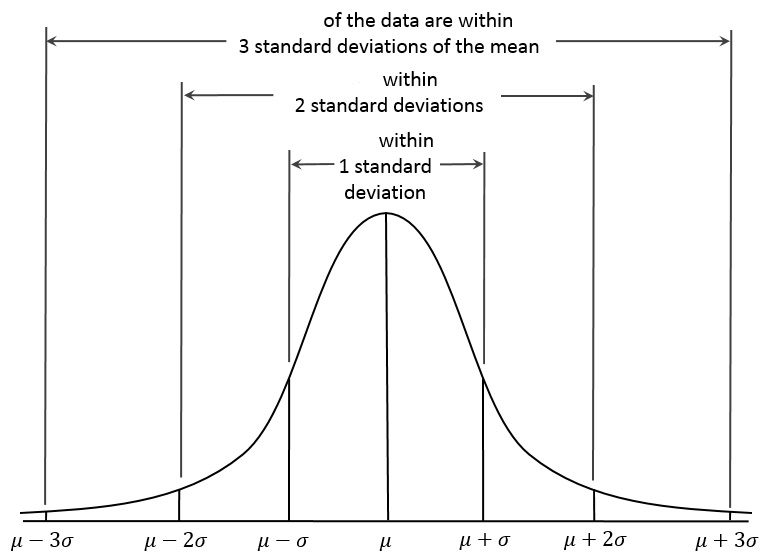
\includegraphics[width=\linewidth]{Gaussian_distribution.jpg}
\end{figure}

\forceindent \textbf{?} How is the distribution depicted above called? What theorem makes it useful for data analysis?

\framebox(347,50){}

\forceindent \textbf{?} A simple random sample of students has a mean age of 25 and \textit{n}=500. Can you calculate the standard error with the information provided? If not, what are you missing?

\framebox(347,50){}

\forceindent \textbf{?} A random sample of 100 students did an IQ test. The resulting average IQ was of 106 with a standard deviation of 16. Can you find a 95 percent confidence interval? (Use the formula below).

\begin{center}
	\scalebox{2}{$\overline{x} \pm Z_{\alpha/2}\times\frac{s}{\sqrt{n}}$}
\end{center}

You can use the above formula to compute any confidence interval. The suffix $\alpha$ (alpha) denotes the confidence level. $Z_{\alpha/2}$ is the critical level for a given alpha. Remember that a critical level of a 95 percent confidence interval is about 1.96. For a 95 percent confidence interval the value of alpha is of 0.05 (because $1-0.95=0.05$). Using this information try to calculate the confidence interval for the exercise above.

\framebox(347,130){}

\forceindent \textbf{?} Can you complete the table below?

\begin{table}[H]
	\centering
	\begin{large}
	\begin{tabular}{ccc}
		\underline{$Z_{\alpha/2}$} & \underline{$\alpha$} & \underline{$1-\alpha$} \\
		1.645          & 0.1          &           \\
		1.96          & 0.05          &           \\
		2.576         &          & 0.99        
	\end{tabular}
	\end{large}
\end{table}

\forceindent \textbf{?} The coffee machine of your university's cafeteria is set up in such way that the average content of a cup of coffee equals a quantity $\mu$. Who knows why but you decided to construct a random sample of 200 cups of coffee. This resulted in an average content of 34cl. Assume your standard deviation was of 6cl. Can you find two confidence intervals one for 90 percent and another for 99 percent?

\framebox(347,150){}


\end{document}
